
\chapter{Introducción}

% --------------------------------------------------------------------------------------------------------------

\section{Descripción del problema}

La antropología es la ciencia que estudia la humanidad en todas sus dimensiones: biológica, cultural, lingüística o arqueológica \cite{AAA2022AnthropologyDefinition}, a lo largo del tiempo y en distintas partes del mundo. La antropología biológica o física se centra en el estudio de la anatomía, el crecimiento, la adaptación y la evolución del cuerpo humano \cite{nawrocki2006}. Dentro de este campo, la \textbf{antropología forense (\acrshort{AF})} es el subcampo especializado que aplica métodos y técnicas antropológicas para resolver cuestiones médico-legales \cite{nawrocki2006}, empleando conocimientos de antropología física, aunque a veces también de la arqueología, para la correcta recuperación y análisis de la evidencia forense.Aunque tradicionalmente asociada al estudio de restos humanos esqueletizados o en descomposición, la \acrshort{AF} también contribuye a la estimación del perfil biológico en individuos vivos, especialmente en contextos legales.

Tradicionalmente, los antropólogos forenses han tenido cinco principales objetivos en su trabajo \cite{byers2023}:

\begin{enumerate}
    
    \item Determinar el \textbf{perfil biológico} de un individuo (es decir, sexo, edad, estatura y ascendencia), ya sea en restos esqueletizados donde los tejidos blandos se han deteriorado hasta el punto de que estas características no pueden determinarse mediante inspección visual, o en personas vivas mediante técnicas no invasivas como análisis radiográficos o morfológicos. 

    \item Identificar la naturaleza de lesiones traumáticas (como heridas de bala, puñaladas o fracturas) en huesos humanos, así como sus causantes, con el objetivo de recopilar información sobre la causa y circunstancias de la muerte.

    \item Estimar el intervalo \textit{post mortem}, es decir, el tiempo transcurrido desde la muerte, gracias a su conocimiento sobre los procesos de descomposición corporal.
    
    \item Asistir en la localización, recuperación y conservación de los restos (superficiales o enterrados) aplicando técnicas arqueológicas, garantizando la recolección de toda la evidencia forense relevante.

    \item Proporcionar información clave para la \textbf{identificación} de los fallecidos, basándose en las características distintivas de los esqueletos.

\end{enumerate}

Además de estos roles, en la actualidad los antropólogos desempeñan otros trabajos que no están relacionados con el ámbito criminalístico. Entre ellos, uno de sus campos de acción más relevantes es la \textbf{identificación de víctimas en contextos de catástrofes masivas} \cite{deBoer2019, prinz2007, beauthier2009}, como accidentes aéreos, ataques terroristas o desastres naturales, donde los restos suelen estar mutilados o desfigurados.

Su labor también es fundamental en la \textbf{recuperación e identificación de violaciones sistemáticas de derechos humanos}, como exterminios, persecuciones políticas y represiones dictatoriales \cite{skinner2003}. Casos como la Guerra Civil Española y la Dictadura Franquista \cite{sanchisgimeno2024, baeta2015}, así como las múltiples dictaduras en el Cono Sur de América \cite{ataliva2024}, han requerido la intervención de equipos forenses para esclarecer la verdad histórica y restituir la identidad de las víctimas a sus familiares, contribuyendo al proceso de memoria, justicia y reparación para las familias afectadas. Esta vinculación con la justicia trasciende lo nacional: la ciencia forense es clave en la \textbf{investigación de crímenes de guerra contra poblaciones civiles}. Organizaciones como Médicos por los Derechos Humanos y la ONU financian equipos especializados que documentan estos crímenes, proporcionando pruebas esenciales para tribunales internacionales \cite{tanaka2020}.

Y por último, también son fundamentales para \textbf{estimar la edad de personas vivas en casos legales}, especialmente cuando no existen registros confiables. Esto ocurre, por ejemplo, en casos de solicitudes de asilo, adopciones internacionales o procesos judiciales donde es necesario determinar si una persona es menor o mayor de edad, lo cual puede tener importantes implicaciones legales. Según el tipo de procedimiento, se puede requerir tanto la estimación de la edad mínima como la edad más probable del individuo, con el fin de priorizar la protección de los menores, evitando que queden expuestos a violaciones de sus derechos.


\subsection{Identificación humana y estimación del perfil biológico}

Como hemos visto, la \textbf{identificación humana (\acrshort{ID})} es una de las principales tareas que aborda la \acrshort{AF}. Consiste en la determinación y verificación de la identidad de una persona en base a \cite{thompson2006}: evidencias circunstanciales (hora y lugar del descubrimiento del cuerpo, efectos personales, confirmación visual por parte de familiares y amigos); y evidencias físicas, obtenidas a través de examinación externa de características como el sexo, color de piel, tatuajes, o huellas dactilares, o, cuando estas no estén disponibles, mediante examinación interna con técnicas médico-científicas, donde se aplican técnicas de antropología y genética forense.

Cabe destacar que, aunque los análisis dactilares y genéticos superan en precisión identificativa a los métodos antropológicos, su aplicabilidad enfrenta limitaciones técnicas significativas que condicionan su uso en ciertos contextos forenses \cite{beauthier2009}. Las huellas dactilares requieren de: tejido blando preservado, lo que es común en cadáveres frescos, pero se pierde con la descomposición o la carbonización; y una base de datos que incluya la huella del individuo en vida (registros \textit{ante mortem}). Por otro lado, en cuanto al análisis genético, este puede verse comprometido por una mala conservación del ADN que puede deberse a su degradación o contaminación. La concentración presente en un cadáver se reduce drásticamente en los primeros 8 meses \textit{post mortem} \cite{higgins2015}, y factores como las altas temperaturas, la exposición a humedad ambiental o la presencia de aguas subterráneas y entornos ricos en oxígeno, que fomentan la presencia microbiana, perjudican la conservación del ADN \cite{latham2018}. Y, aún extraída una secuencia válida de ADN, se necesita de muestras con las que compararla, a ser posible de familiares de primer grado, para establecer una identificación concluyente. 

Por tanto, la \acrshort{AF} contribuye al problema de identificación humana en dos escenarios \cite{swganth2010}:  

\begin{enumerate}

    \item Cuando los otros métodos no son viables, dado que las pruebas no se puedan recoger o no sean válidas, o no haya registros con los que compararlas.
    
    \item Como apoyo a otras técnicas de identificación. Por ejemplo, las técnicas de estimación del perfil biológico pueden reducir el grupo de posibles coincidencias en bases de datos genéticos, facilitando el cotejo de secuencias genéticas y reduciendo el coste del proceso.  

\end{enumerate}

La \textbf{estimación del perfil biológico (\acrshort{PB})} es, por tanto, un proceso fundamental de la \acrshort{AF}, en el cual se determinan características biológicas clave de un individuo \cite{byers2023}: 

\begin{itemize}

    \item \textbf{sexo}, mediante el análisis morfológico y métrico de rasgos sexuales en el esqueleto, 
    especialmente en la pelvis y el cráneo;
    
    \item \textbf{edad}, estimada a partir de cambios morfológicos y de desarrollo en el esqueleto, pudiendo referirse tanto a la \textbf{edad al momento de la muerte} en restos óseos, como a la \textbf{edad cronológica}%
    \footnote{
        La edad cronológica es la edad real de una persona desde su nacimiento, mientras que la edad biológica o fisiológica refleja la condición fisiológica del cuerpo \cite{marcante2025}.
    }
    en personas vivas en contextos forenses o humanitarios;
    
    \item \textbf{estatura}, mediante la estimación de la talla a partir de longitudes óseas, particularmente de los huesos largos; y
    
    \item \textbf{ascendencia} o \textbf{afinidad poblacional}, analizando variaciones craneométricas y morfológicas asociadas a poblaciones o grupos geográficos (actualmente en revisión \cite{ross2021a, ross2021b, flouri2022}).

\end{itemize}

En los problemas de \acrshort{ID}, cuando estas características biológicas coinciden con los registros \textit{ante mortem}, se fortalece la hipótesis de identificación; en cambio, si existen una o más discrepancias ---especialmente de alguna característica firme como múltiples epífisis no fusionadas, que no pueden ocurrir en un adulto mayor---, el individuo es excluido como posible coincidencia \cite{byers2023}. En la Figura \ref{fig:SFI_pipeline} podemos observar que la estimación del \acrshort{PB} es uno de los primeros pasos en el proceso de \acrshort{ID} forense. 

\begin{figure}[htbp]
    \centering
    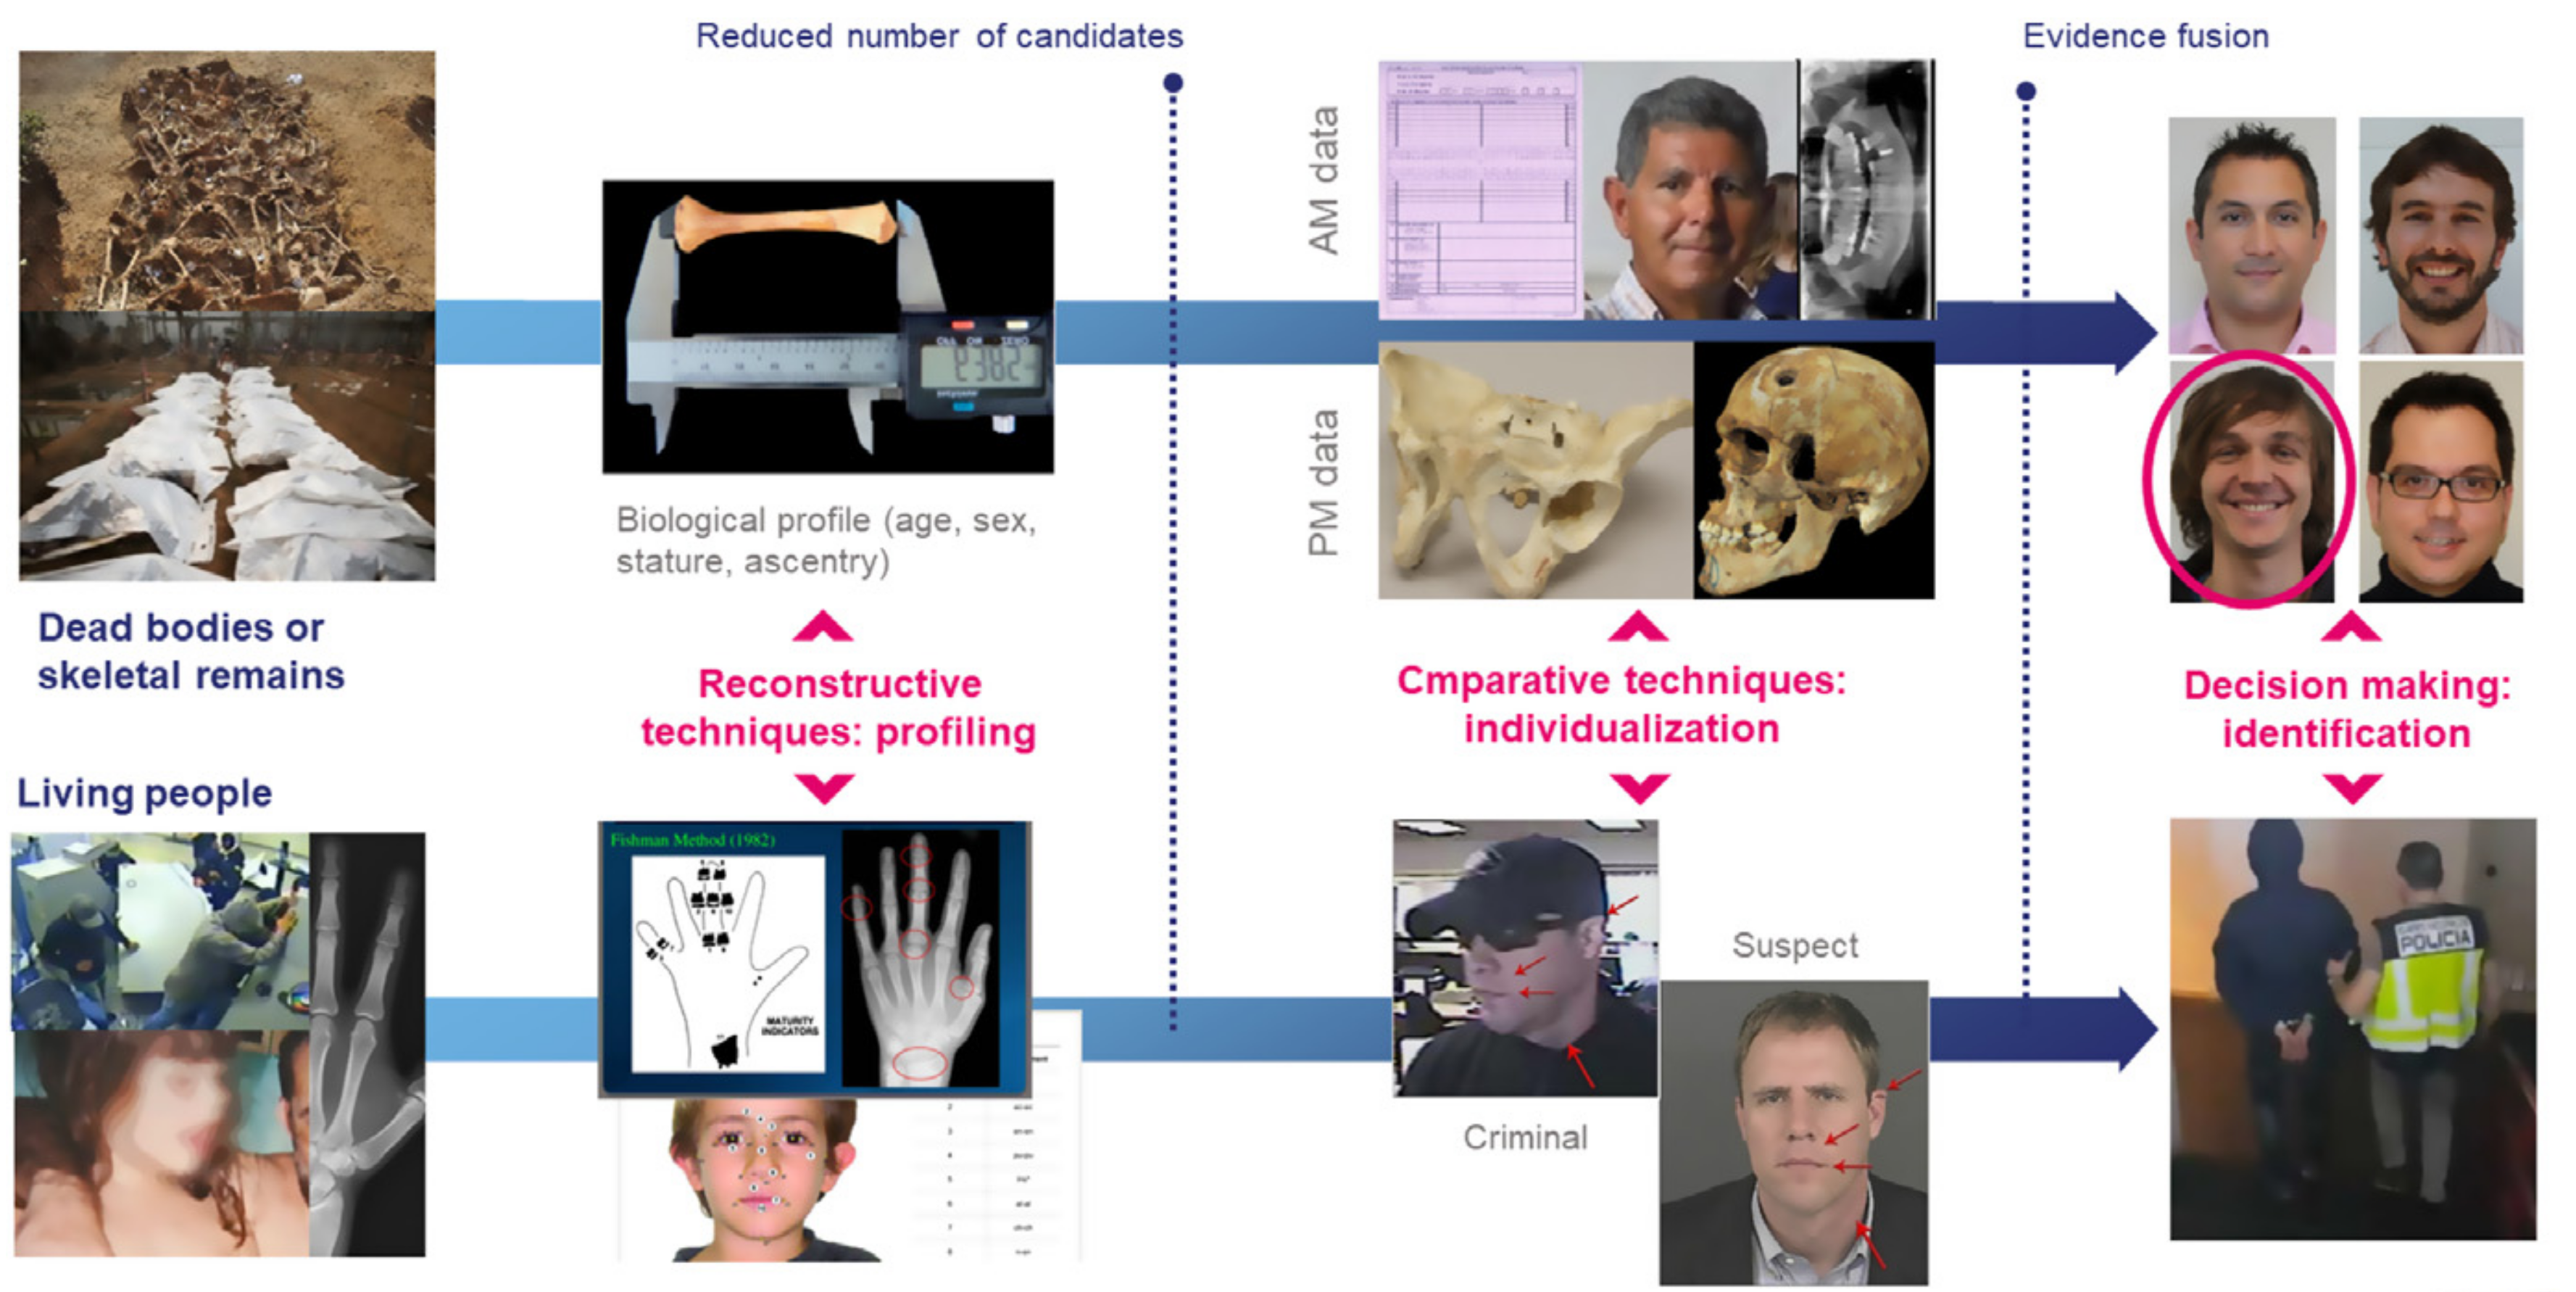
\includegraphics[width=\textwidth]{capitulos/cap_01/imagenes/SFI_pipeline.png}
    \caption[
        Procedimiento secuencial para la identificación forense basada en el esqueleto humano (\textit{skeleton-based forensic identification}).
    ]{
        Procedimiento secuencial para la identificación forense basada en el esqueleto humano (\textit{skeleton-based forensic identification}) \cite{mesejo2020}.
    } 
    \label{fig:SFI_pipeline}
\end{figure}

La estimación del \acrshort{PB} en restos humanos es una tarea compleja, especialmente cuando se estima la edad en el momento de la muerte, ya que hay diferentes métodos a aplicar dependiendo de la fase de desarrollo del individuo. Las variaciones en la morfología de los huesos son bien conocidas, pero estas no siempre ocurren al mismo tiempo en diferentes individuos, ya que no están expuestos a las mismos condiciones genéticas y del entorno.

Además, como se ha mencionado anteriormente, la estimación de edad también se realiza sobre personas vivas en casos legales donde la edad es un factor determinante \cite{schmeling2016}, por ejemplo, con menores migrantes no acompañados. En estos casos no se tiene acceso a los huesos de la persona de forma directa, por lo que el análisis se realiza sobre imágenes médicas.

% ------------------------------------------------------------------------------------------------------------
% ------------------------------------------------------------------------------------------------------------
% ------------------------------------------------------------------------------------------------------------

\section{Motivación}

Los métodos de estimación del \acrshort{PB} se basan en la evaluación visual y en el análisis morfométrico de rasgos esqueléticos, que requieren de conocimiento especializado. Sin embargo, su aplicación puede presentar ambigüedades en su formulación que den lugar a interpretaciones variables ---muchas veces fruto de sesgos cognitivos \cite{nakhaeizadeh2014, cooper2019}--- y están sujetos a posibles errores de medición \cite{langley2018}. Además, la gran variabilidad genética y ambiental entre individuos, que afecta la morfología del esqueleto y genera diferencias significativas entre poblaciones de distintas regiones \cite{ubelaker2017}, hace que muchos de estos métodos ---basados en muestras de referencia limitadas o no representativas de la diversidad humana global--- pierdan precisión. Esto puede introducir sesgos al estimar el \acrshort{PB} de individuos de grupos poco estudiados o con características atípicas.

Frente a estas limitaciones, recientes avances en inteligencia artificial (\acrshort{IA}) y \textit{machine learning} (\acrshort{ML}) han demostrado el potencial de mejorar la exactitud y objetividad de estimación del \acrshort{PB}, tanto para la estimación de sexo \cite{curate2017, darmawan2015, pinto2016} como de edad \cite{kim2017, larson2018, lee2017}.

Sin embargo, aún mejorando la exactitud de las predicciones, los modelos siguen mostrando carencias respecto a la cuantificación de incertidumbre, pues no todas las predicciones tienen el mismo nivel de confianza o fiabilidad. Ya en \cite{ferrante2009} se introducía no solo la necesidad de identificar el método adecuado para estimar la edad a partir de los elementos disponibles, sino también de evaluar su confiabilidad y realizar un estudio del error arrojado por las predicciones del método. Estos generalmente se han basado en la estadística frecuentista%
\footnote{
    La estadística frecuentista es la corriente que se desarrolla a partir de los conceptos de probabilidad y que se centra en el cálculo de probabilidades y el contraste de hipótesis.
}
\cite{verma2020, stepanovsky2024, heinrich2024}. Un ejemplo de este tipo de análisis se ilustra en la Figura \ref{fig:regression_lentibia_stature}, donde se examina la distribución probabilística del error residual arrojado por un modelo de regresión.

\begin{figure}[h]
    \centering
    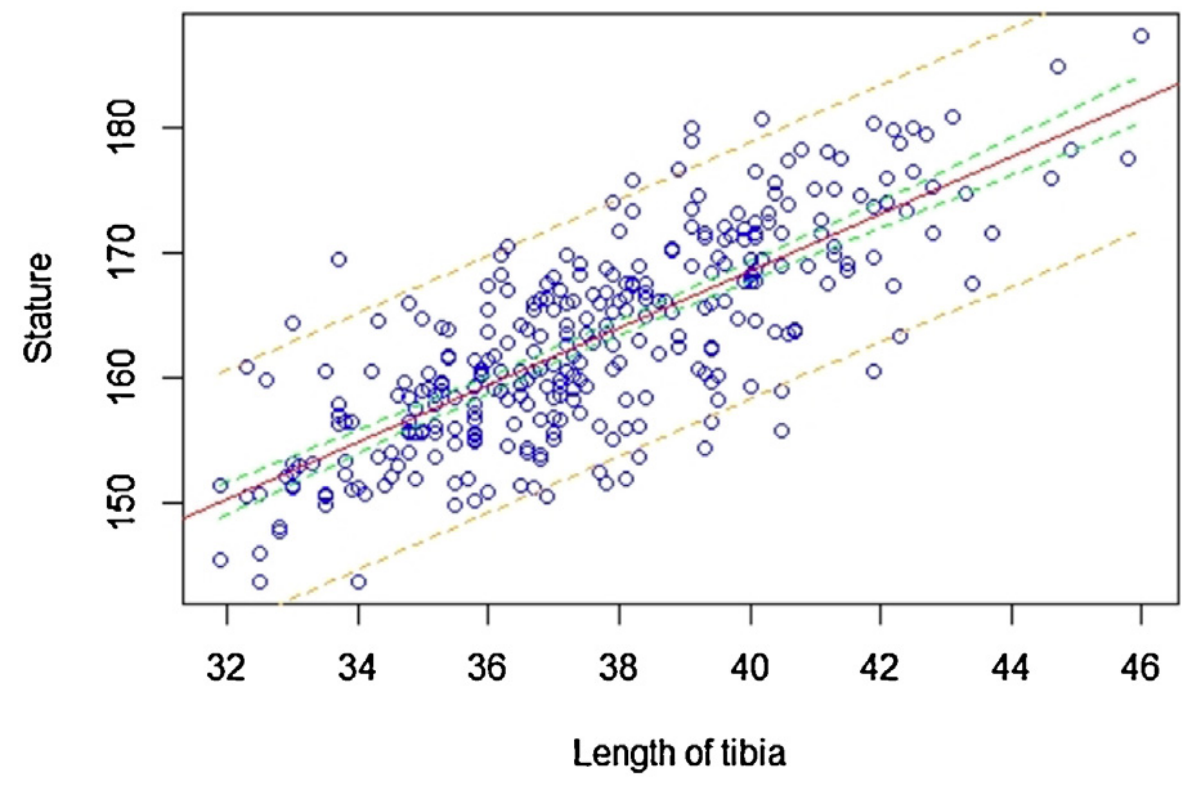
\includegraphics[width=0.75\textwidth]{capitulos/cap_01/imagenes/regression_line_lentibia_stature.png}
    \caption[
        Línea de regresión de un modelo de regresión que predice la estatura a partir de la longitud de la tibia.
    ]{
        Línea de regresión del modelo de regresión propuesto en \cite{verma2020} que predice la estatura a partir de la longitud de la tibia. En rojo, la línea de regresión; en verde, los intervalos de confianza al 95\% para la media poblacional; y la naranja, los intervalos de predicción al 95\% de confianza. Aunque en ambos casos se utilice la palabra ``confianza'', se refieren a conceptos distintos: el intervalo de confianza indica el rango donde, con una probabilidad del 95\%, se espera que se encuentre la media poblacional estimada para un valor dado de la variable independiente, mientras que el intervalo de predicción señala el rango donde, con la misma probabilidad, podría ubicarse una observación individual futura. Consulte el Anexo \ref{chap:intervalos_valores_razonables} para entrar en detalle.
    } 
    \label{fig:regression_lentibia_stature}
\end{figure}

Aunque existen métricas para evaluar el error cuando se dispone de \textit{ground truth}, la mayoría de los modelos actuales se limitan a ofrecer predicciones puntuales en regresión \cite{park2024, imaizumi2021, stepanovsky2024} o etiquetas únicas en clasificación \cite{venema2022, park2024}, sin cuantificar la incertidumbre asociada a cada predicción.

Con lo anterior se expone la motivación de la aplicación de \acrshort{ML} a la \acrshort{AF}, así como de la necesidad de cuantificar la incertidumbre en las predicciones, para ofrecer garantías de confiabilidad estadística que aspiren a sustentar la validez legal en contextos judiciales. Algunos datos que magnifican la necesidad de técnicas de \acrshort{AF} confiables actualmente son:

% 1/3 de los muertos del 11S sin identificar

\begin{itemize}

    \item En los últimos años, ha aumentado significativamente el número de cadáveres hallados en el territorio español, como podemos apreciar en la Figura \ref{fig:evolucion_hallazgosID_cadaveres} \cite{interior2025desaparecidos}. En 2024 se ha alcanzado una cifra record, ---en gran parte debido a las inundaciones de la DANA Valencia del mismo año---, de 531 cadáveres en 2024, de los cuales se pudo identificar a 323.

    \begin{figure}[h]
        \centering
        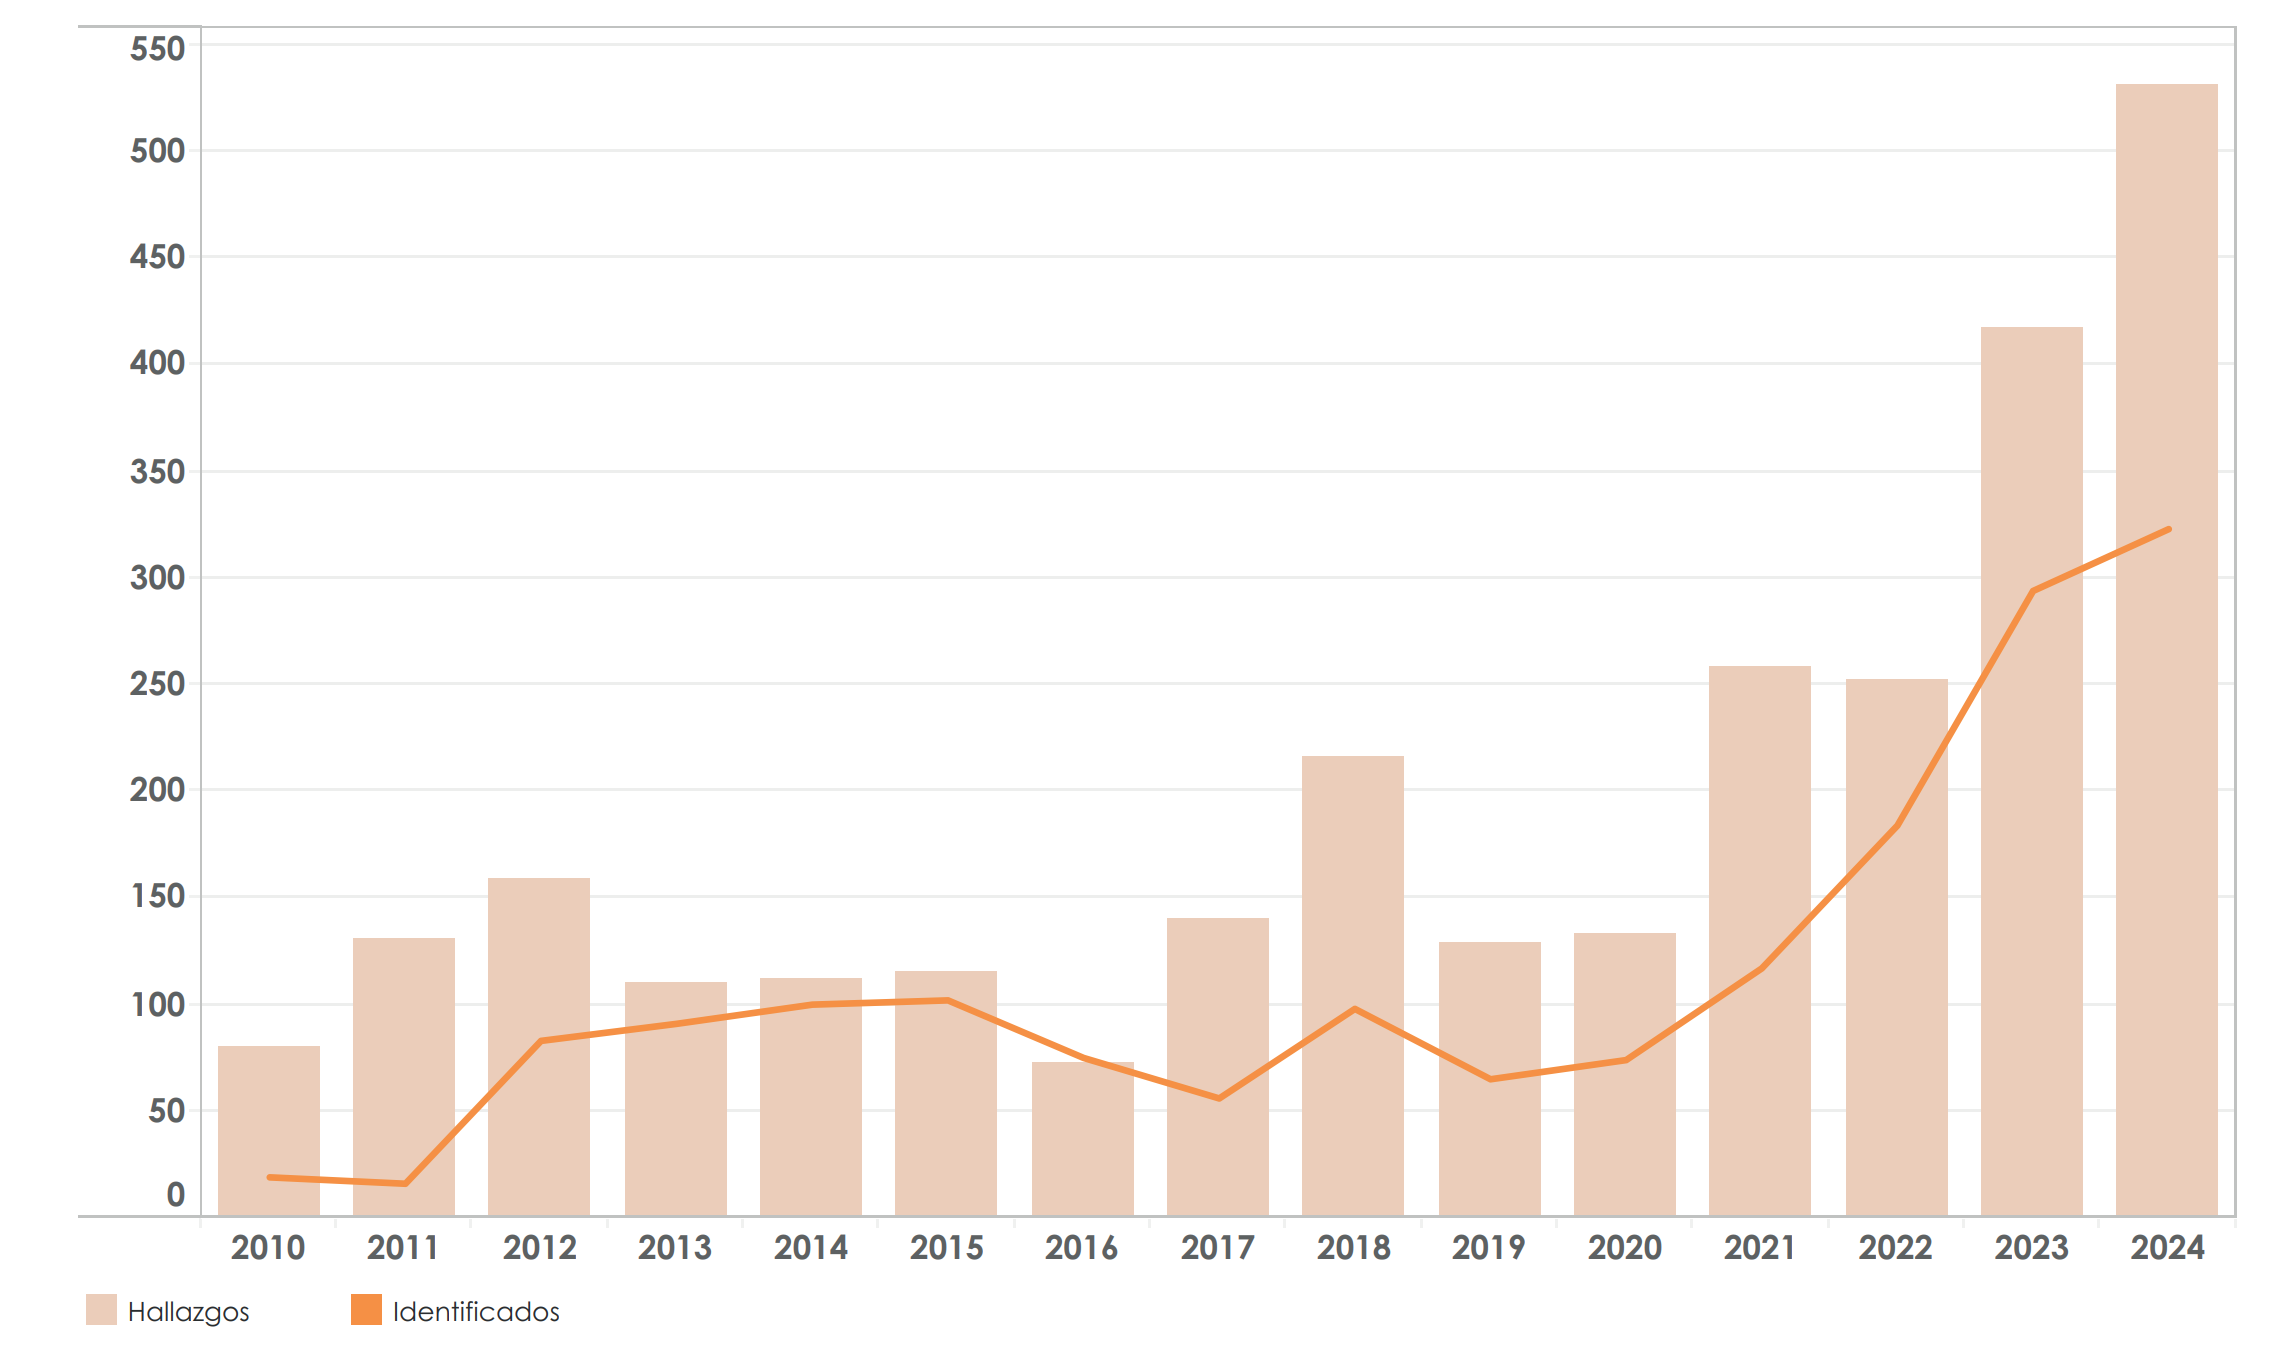
\includegraphics[width=0.8\textwidth]{capitulos/cap_01/imagenes/hallazgos_cadaveres.png}
        \caption[
            Evolución de hallazgos/identificación de cadáveres en España (2010-2024).
        ]{
            Evolución de hallazgos/identificación de cadáveres en España (2010-2024) \cite{interior2025desaparecidos}. 
        } 
        \label{fig:evolucion_hallazgosID_cadaveres}
    \end{figure}

    \item En 2020, de las 2.457 fosas totales documentadas de la Guerra Civil y el franquismo, aún 1.221 seguían sin ser intervenidas y se estimaba que ``con una intervención oficial del Estado podrían recuperarse unos 20 a 25.000 individuos'' e identificar ``entre 5 y 7.000 de ellos'', estimándose  necesario contar con unos 40-50 profesionales de la antropología forense \cite{etxeberria2020}. 

    % \item De acuerdo con UNICEF \cite{unicef2013}, en 2012 cerca de 230 millones de niños menores de cinco años no contaban con un registro oficial de nacimiento. Las regiones con las tasas más bajas de registro incluyen África subsahariana (44\%) y el sur de Asia (39\%). Esta situación se agrava aún más, ya que muchos niños registrados no poseen un certificado de nacimiento, y los documentos existentes suelen perderse durante procesos de migración.

    \item En España, se ha registrado en la última década (2013-2023) un aumento significativo en la llegada de Menores Extranjeros No Acompañados \cite{fge2024,fge2019,fge2016,fge2013}, que ha disparado consigo el número de diligencias abiertas para la determinación de su edad, como se ve reflejado en la Figura \ref{fig:evolucion_DPDE}.

    \begin{figure}[h]
        \centering
        \includegraphics[width=0.8\textwidth]{capitulos/cap_01/imagenes/dpde_España.png}
        \caption[
            Evolución del número de diligencias preprocesales de determinación de edad abiertas en España (2011-2023).
        ]{
            Evolución del número de diligencias preprocesales de determinación de edad abiertas en España (2011-2023). Elaboración propia a partir de \cite{fge2013,fge2016,fge2019, fge2024}.
        } 
        \label{fig:evolucion_DPDE}
    \end{figure}

    \item La relevancia de la ciencia forense en la identificación de víctimas y la protección de la dignidad humana ha convertido su aplicación en un pilar fundamental de los derechos humanos y la justicia internacional, naciendo así la  \textbf{acción forense humanitaria} \cite{cordner2017}. Esta disciplina emplea la ciencia forense con un propósito exclusivamente humanitario, con los objetivos de: identificar a las personas fallecidas, gestionar dignamente sus restos y aliviar el sufrimiento de sus familias en situaciones de conflicto, migración y desastres naturales \cite{tidballbinz2021}. 

\end{itemize}

% ------------------------------------------------------------------------------------------------------------

\section{Objetivos}

La \textbf{predicción conformal} emerge como un marco teórico robusto para generar intervalos de predicción con garantías estadísticas sólidas, independientemente de la distribución subyacente de los datos. A diferencia de los enfoques tradicionales, este método no solo ofrece predicciones puntuales sino que cuantifica la incertidumbre asociada a cada estimación mediante intervalos o conjuntos de predicción que reflejan la confiabilidad de la predicción en cada caso particular.

Este Trabajo de Fin de Grado tiene un doble objetivo: 

\begin{itemize}

    \item desde un prisma teórico, defender la cuantificación de incertidumbre como herramienta esencial en \acrshort{ML}, ofrecer un panorama de métodos destacados, analizando sus ventajas y limitaciones, y centrarnos en la predicción conformal y sus técnicas más populares.

    \item aplicar la predicción conformal a un contexto práctico como es el problema de estimación del \acrshort{PB}, centrándose en la estimación de edad y de sexo a partir de datos biológicos e imágenes médicas.

\end{itemize}

De esta forma, podremos incorporar la incertidumbre propia del problema a resolver y del modelo entrenado para él, para, en aquellos casos más confusos, devolver conjuntos de predicciones con más de una etiqueta predicha (p.ej., \{masculino, femenino\}) en problemas de clasificación, o intervalos de predicción más amplios (p.ej., edad$\in$[16,20]) en problemas de regresión, en ambos casos para un nivel de confianza determinado.
Por tanto, podemos desgranar los objetivos en:

\begin{itemize}

    \item Estudiar de forma exhaustiva la bibliografía sobre predicción conformal y algunas de sus técnicas,así como de la estimación de sexo y edad.

    \item Implementar, entrenar y validar modelos de regresión ---en problemas de estimación de edad--- y clasificación ---tanto en problema de estimación de sexo como edad legal--- a los que aplicar la inferencia conformal, y comparar aproximaciones heurísticas de cuantificación de incertidumbre con los métodos conformales.
    
    % \item s intervalos y conjuntos de predicciones generados para evaluar su calibración empírica y utilidad forense.  

    \item Realizar una primera aproximación a un marco interpretable y con garantías estadísticas para la estimación del perfil biológico (véase un ejemplo práctico en la Figura \ref{fig:example_intervalic_estimation}), donde la incertidumbre cuantificada pueda integrarse en informes periciales bajo estándares jurídicos.

\end{itemize}


\begin{figure}[htbp]
    \centering
    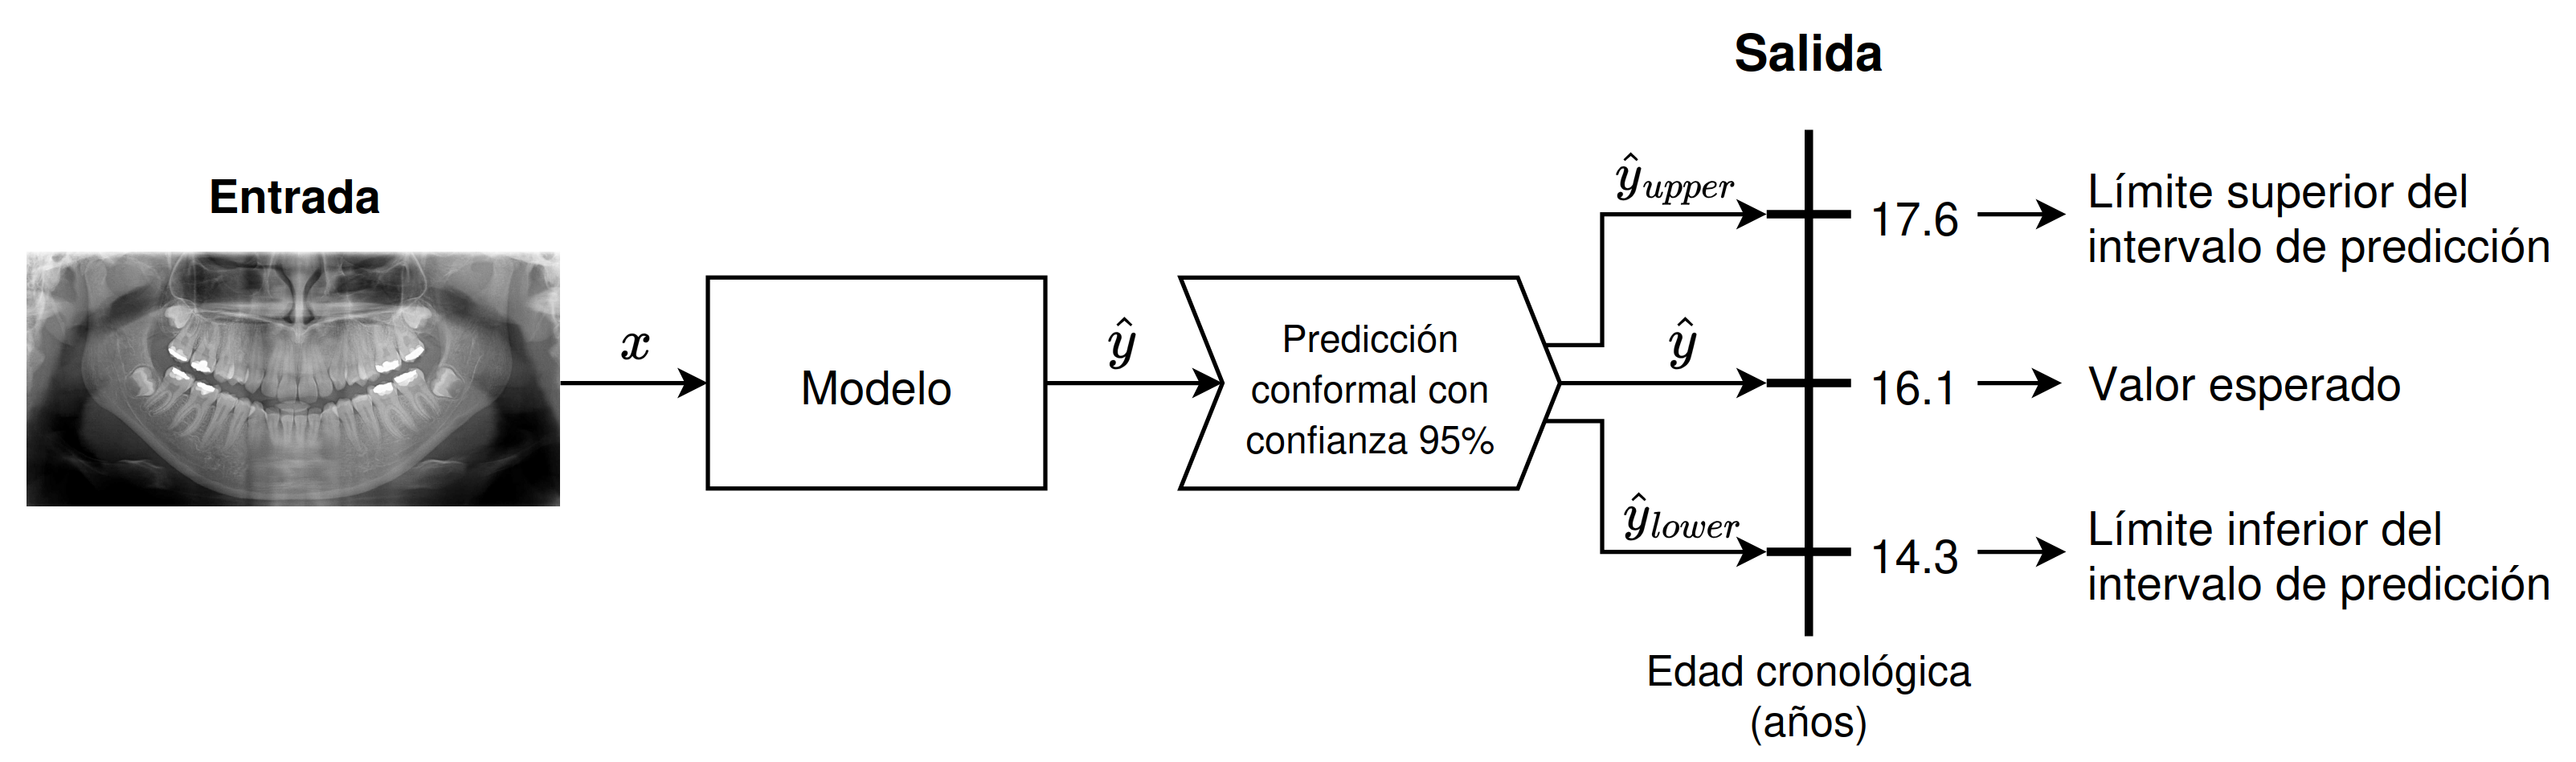
\includegraphics[width=\textwidth]{capitulos/cap_01/imagenes/example_intervalic_estimation.png}
    \caption[
        Diagrama de modelo de regresión que usa predicción conformal, el cual, además de proporcionar una estimación puntual del valor esperado, entrega un intervalo de predicción con un nivel de confianza del 95\%.
    ]{ 
        Diagrama de modelo de regresión que usa predicción conformal, el cual, además de proporcionar una estimación puntual del valor esperado, entrega un intervalo de predicción con un nivel de confianza del 95\%.
        Esta salida se lee de la siguiente manera: ``la edad esperada del individuo es de 16.1 años y, con una confianza del 95\%, la edad real del individuo está entre los 14.3 y los 17.6 años''.
    } 
    \label{fig:example_intervalic_estimation}
\end{figure}


En resumen, este trabajo pretende explorar la integración de marcos probabilísticos en la práctica forense que capturen la incertidumbre de los problemas, y facilitar el uso de la inferencia conformal en ellos. Este enfoque proporciona estimaciones calibradas de incertidumbre, con garantías estadísticas de contener el valor real en un conjunto o intervalo de predicción, útiles para la toma de decisiones fundamentadas en contextos prácticos donde la interpretabilidad y robustez son críticas.

% ------------------------------------------------------------------------------------------------------------

\section{Planificación temporal}

Partimos de que el Proyecto de Fin de Grado tiene asignado 12 créditos ECTS, lo que equivale a 360 horas de trabajo%
\footnote{
    De 25 a 30 horas por crédito según \cite{ComisionEuropea2015ECTS}.
}. Estas 360 horas se distribuyen a lo largo del segundo cuatrimestre del curso 2024/2025, constando de 66 días lectivos, lo que resulta en una carga de trabajo de aproximadamente 5.45 horas al día, aproximadamente 5 horas y media. La planificación inicial del proyecto se presenta en el diagrama de Gantt de la Figura \ref{fig:inicial_gantt}.


% \begin{landscape}
% \thispagestyle{fancy}
% \begin{figure}
%     \centering
%     \begin{ganttchart}[
%         expand chart=\linewidth,
%         hgrid,
%         x unit=1.15mm,
%         y unit chart=6.5mm,
%         y unit title=10mm,
%         time slot format=isodate,
%         %
%         bar/.append style={draw=black!50, fill=black!20},
%         bar label font=\small,
%         bar top shift = 0.2,
%         bar height = 0.55,
%         %
%         group/.append style={draw=black, fill=green!50},
%         %
%         milestone/.append style={fill=orange, rounded corners=3pt},
%         % group label font=\small\bfseries,    % texto de grupos más pequeño y en negrita
%         % milestone label font=\footnotesize
%     ]{2025-02-17}{2025-06-30}
%         \gantttitlecalendar{year, month=shortname}\\
%         \ganttbar{Definición de propuesta y objetivos}{2025-02-17}{2025-02-19} \\
%         \ganttbar{Implementación del núcleo}{2025-02-20}{2025-03-09} \\
%         \ganttbar{Implementación de algoritmos de CP}{2025-03-10}{2025-04-13} \\
%         \ganttbar{Experimentación}{2025-04-14}{2025-06-08} \\
%         \ganttbar{Análisis de resultados}{2025-06-09}{2025-06-22} \\
%         \ganttbar{Redacción de la memoria}{2025-02-20}{2025-06-22}\\
%         \ganttbar{Contingencia}{2025-06-23}{2025-06-30}
%     \end{ganttchart}
%     \caption{Diagrama de Gantt inicial del proyecto}
%     \label{fig:inicial_gantt}
% \end{figure}

% \begin{figure}
%     \centering
%     \begin{ganttchart}[
%         expand chart=\linewidth,
%         title label font=\small,
%         hgrid,
%         x unit=1.15mm,
%         y unit chart=6.5mm,
%         y unit title=10mm,
%         time slot format=isodate,
%         %
%         bar/.append style={draw=black!50, fill=black!20},
%         bar label font=\small,      % texto de tareas más pequeño
%         bar top shift = 0.2,
%         bar height = 0.55,
%         %
%         group/.append style={draw=black, fill=black!100},
%         % group label font=\small\bfseries,    % texto de grupos más pequeño y en negrita
%         %
%         % milestone label font=\footnotesize
%         milestone/.append style={draw=black, fill=black},
%         milestone left shift =-0.5,
%         milestone right shift =1.5,
%         milestone label font=\footnotesize,
%         milestone inline label node/.append style={left=1ex,text opacity=1},
%         flip/.style={milestone inline label node/.append style={right=2ex}},
%     ]{2025-02-17}{2025-08-31}
%         \gantttitlecalendar{year, month=shortname}\\
%         \ganttbar{Definición de propuesta y objetivos}{2025-02-24}{2025-02-26} \\
%         %
%         \ganttbar{Implementación del núcleo}{2025-03-15}{2025-05-16}
%         \ganttbar[inline]{Revisión}{2025-06-19}{2025-06-28} \\
%         %
%         \ganttbar{Implementación de técnicas de CP}{2025-02-27}{2025-03-14}
%         \ganttbar[inline]{Regres.}{2025-05-28}{2025-07-06} 
%         \ganttbar[inline]{Clasif.}{2025-07-07}{2025-08-01} \\
%         %
%         \ganttbar{Experimentación}{2025-07-14}{2025-08-03}
%         \ganttbar[inline]{}{2025-06-15}{2025-07-06} \\
%         %
%         \ganttbar{Análisis de resultados}{2025-07-18}{2025-08-15}\\
%         %
%         \ganttbar{Redacción de la memoria}{2025-02-27}{2025-08-22} 
%         \ganttmilestone[inline]{Cap.1}{2025-05-02} 
%         \ganttmilestone[inline]{Cap.2}{2025-06-03} 
%         \ganttmilestone[inline]{Cap.3-4}{2025-07-06}
%         \ganttmilestone[inline]{Cap.5-6}{2025-08-22}
%     \end{ganttchart}
%     \caption{Diagrama de Gantt final del proyecto}
%     \label{fig:final_gantt}
% \end{figure}
% \end{landscape}


% \begin{figure}
%     \centering
%     \begin{ganttchart}[
%         expand chart=\linewidth,
%         hgrid,
%         x unit=1.15mm,
%         y unit chart=6.5mm,
%         y unit title=10mm,
%         time slot format=isodate,
%         %
%         bar/.append style={draw=black!50, fill=black!20},
%         bar label font=\small,
%         bar top shift = 0.2,
%         bar height = 0.55,
%         %
%         group/.append style={draw=black, fill=green!50},
%         %
%         milestone/.append style={fill=orange, rounded corners=3pt},
%         % group label font=\small\bfseries,    % texto de grupos más pequeño y en negrita
%         % milestone label font=\footnotesize
%     ]{2025-02-17}{2025-06-30}
%         \gantttitlecalendar{year, month=shortname}\\
%         \ganttbar{Definición de propuesta y objetivos}{2025-02-17}{2025-02-19} \\
%         \ganttbar{Implementación del núcleo}{2025-02-20}{2025-03-09} \\
%         \ganttbar{Implementación de algoritmos de CP}{2025-03-10}{2025-04-13} \\
%         \ganttbar{Experimentación}{2025-04-14}{2025-06-08} \\
%         \ganttbar{Análisis de resultados}{2025-06-09}{2025-06-22} \\
%         \ganttbar{Redacción de la memoria}{2025-02-20}{2025-06-22}\\
%         \ganttbar{Contingencia}{2025-06-23}{2025-06-30}
%     \end{ganttchart}
%     \caption{Diagrama de Gantt inicial del proyecto}
%     \label{fig:inicial_gantt}
% \end{figure}

\begin{figure}[h]
    \centering
    \begin{ganttchart}[
        expand chart=\linewidth,
        title label font=\footnotesize,
        hgrid,
        x unit=1.15mm,
        y unit chart=6.5mm,
        y unit title=10mm,
        time slot format=isodate,
        %
        bar/.append style={draw=black!50, fill=black!20},
        bar label font=\footnotesize,      % texto de tareas más pequeño
        bar top shift = 0.2,
        bar height = 0.55,
        %
        group/.append style={draw=black, fill=green!50},
        %
        milestone/.append style={fill=orange, rounded corners=3pt},
        % group label font=\small\bfseries,    % texto de grupos más pequeño y en negrita
        % milestone label font=\footnotesize
    ]{2025-02-17}{2025-06-30}
        \gantttitlecalendar{year, month=shortname}\\
        \ganttbar{Definición de propuesta y objetivos}{2025-02-17}{2025-02-19} \\
        \ganttbar{Implementación del núcleo}{2025-02-20}{2025-03-09} \\
        \ganttbar{Implementación de algoritmos de CP}{2025-03-10}{2025-04-13} \\
        \ganttbar{Experimentación}{2025-04-14}{2025-06-08} \\
        \ganttbar{Análisis de resultados}{2025-06-09}{2025-06-22} \\
        \ganttbar{Redacción de la memoria}{2025-02-20}{2025-06-22}\\
        \ganttbar{Contingencia}{2025-06-23}{2025-06-30}
    \end{ganttchart}
    \caption{Diagrama de Gantt inicial del proyecto}
    \label{fig:inicial_gantt}
\end{figure}

No obstante, debido a ajustes en la orientación conceptual del trabajo, modificaciones en el enfoque metodológico y determinadas circunstancias personales de salud, fue necesario realizar cambios sobre la planificación inicial, posponiéndose finalmente la entrega del trabajo al mes de septiembre.

\begin{figure}[h]
    \centering
    \begin{ganttchart}[
        expand chart=\linewidth,
        title label font=\footnotesize,
        hgrid,
        x unit=1.15mm,
        y unit chart=6.5mm,
        y unit title=10mm,
        time slot format=isodate,
        %
        bar/.append style={draw=black!50, fill=black!20},
        bar label font=\footnotesize,      % texto de tareas más pequeño
        bar top shift = 0.2,
        bar height = 0.55,
        %
        group/.append style={draw=black, fill=black!100},
        % group label font=\small\bfseries,    % texto de grupos más pequeño y en negrita
        %
        % milestone label font=\footnotesize
        milestone/.append style={draw=black, fill=black},
        milestone label font=\footnotesize,
        milestone left shift =-1.7,
        milestone right shift =2.5,
        milestone inline label node/.append style={left=0.5ex,text opacity=1},
        flip/.style={milestone inline label node/.append style={right=2ex}},
    ]{2025-02-17}{2025-08-31}
        \gantttitlecalendar{year, month=shortname}\\
        \ganttbar{Definición de propuesta y objetivos}{2025-02-24}{2025-02-26} \\
        %
        \ganttbar{Implementación del núcleo}{2025-03-15}{2025-05-16}
        \ganttbar[inline]{Revisión}{2025-06-19}{2025-06-28} \\
        %
        \ganttbar{Implementación de técnicas de CP}{2025-02-27}{2025-03-14}
        \ganttbar[inline]{Regres.}{2025-05-28}{2025-07-06} 
        \ganttbar[inline]{Clasif.}{2025-07-07}{2025-08-01} \\
        %
        \ganttbar{Experimentación}{2025-07-14}{2025-08-03}
        \ganttbar[inline]{}{2025-06-15}{2025-07-06} \\
        %
        \ganttbar{Análisis de resultados}{2025-07-18}{2025-08-15}\\
        %
        \ganttbar{Redacción de la memoria}{2025-02-27}{2025-08-22} 
        \ganttmilestone[inline]{Cap.1}{2025-05-02} 
        \ganttmilestone[inline]{Cap.2}{2025-06-03} 
        \ganttmilestone[inline]{Cap.3-4}{2025-07-10}
        \ganttmilestone[inline]{Cap.5-6}{2025-08-22}
    \end{ganttchart}
    \caption{Diagrama de Gantt final del proyecto}
    \label{fig:final_gantt}
\end{figure}

La organización temporal del trabajo se desarrolló finalmente de la siguiente manera (véase la Figura \ref{fig:final_gantt}): 

\begin{itemize}

    \item Febrero: se redactó la propuesta del proyecto, la cual fue aceptada en el plazo de una semana.
    
    \item Marzo: la primera parte del mes se destinó a la implementación de algunas técnicas de predicción conformal en clasificación(\acrshort{LAC}, \acrshort{APS} y \acrshort{RAPS}) sobre el conjunto de datos CIFAR-10. A mediados de mes se concedió acceso al clúster SLURM, lo que permitió comenzar la organización del proyecto, la implementación del núcleo del código y la configuración del entorno de trabajo mediante un proceso iterativo de prueba y error orientado a obtener una solución más cómoda y flexible.
    
    \item Abril: se llevó a cabo la búsqueda, revisión, organización y análisis de bibliografía, con especial atención a la literatura en \acrshort{AF}. A mediados de mes se obtuvo acceso al conjunto de datos definitivo que sería utilizado en el proyecto. Fue necesario adaptar el núcleo de código previamente desarrollado, dedicándose varias semanas a la experimentación y mejora del modelo de red neuronal convolucional. Se aprovechó para organizar el código y subirlo a un repositorio. 

    \item Mayo: a principios de mes se completó una primera versión del capítulo inicial (\textit{Introducción}). Durante la primera mitad del mes se continuó con la optimización del entrenamiento e inferencia del modelo, en paralelo con la redacción del capítulo de Fundamentos teóricos.

    \item Junio: a comienzos de mes se obtuvo la primera versión completa del capítulo segundo (\textit{Fundamentos teóricos}). En este momento se decidió centrar los esfuerzos en la parte de regresión, lo que condujo a la implementación de las técnicas de \acrshort{CP} aplicadas a este contexto. Durante el proceso se identificó la necesidad de reformar nuevamente el núcleo del código, con el fin de reducir repeticiones y dotarlo de mayor flexibilidad, permitiendo mediante argumentos entrenar toda la red o únicamente la cabeza, seleccionar la técnica de \acrshort{CP}, realizar inferencia, entre otras opciones. De forma paralela, se avanzó en la redacción del capítulo tercero (\textit{Estado del arte}) y del capítulo cuarto (\textit{Materiales y métodos}).

    \item Julio: a principios de mes se dispuso de una versión preliminar de la memoria que incluía la parte de regresión hasta la presentación de resultados, aunque sin discusión. Tras esto, el trabajo se orientó hacia la implementación de técnicas de \acrshort{CP} para clasificación, en problemas derivados del enfoque de regresión. Asimismo, se desarrolló un sistema de almacenamiento más organizado de los resultados, de manera que pudieran ser cargados posteriormente en un cuaderno Jupyter para su análisis.

    \item Agosto: se discutieron los resultados obtenidos tanto en regresión como en clasificación, se completaron apartados pendientes de la memoria y se llevaron a cabo ajustes finales. Finalmente, se redactó la conclusión y el \textit{abstract}.
    
\end{itemize}

Finalmente, el trabajo se desarrolló entre el 24 de febrero y el 22 de agosto, considerando únicamente los días laborables, con excepción de los periodos del 4 al 8 de junio y del 3 al 10 de agosto, debido a vacaciones. Durante los días laborables se dedicó una media de 6 horas diarias, mientras que los sábados se trabajó aproximadamente 3 horas diarias%
\footnote{Estimación realizada de manera aproximada.}.

Teniendo en cuenta esta distribución, se puede estimar el total de horas trabajadas de la siguiente manera:

\begin{itemize}
    \item Días laborables efectivos: $122\textnormal{ días} \times 6\textnormal{h/día} = 732\textnormal{h}$
    \item Sábados: $23\textnormal{ días} \times 3\textnormal{h/día} = 69\textnormal{h}$
\end{itemize}

Por tanto, el total aproximado de horas dedicadas al proyecto asciende a 801 horas, lo que supera por mucho la cifra teórica de 360 horas. Este tiempo de más se puede atribuir a varias causas principales: 

\begin{itemize}

    \item Complejidad del proyecto: Nunca antes me había enfrentado a un trabajo de esta complejidad, por lo que la planificación inicial no podía anticipar todas las dificultades técnicas y conceptuales.
    
    \item Adaptación y organización del código: La necesidad de modificar constantemente el núcleo del código para hacerlo más modular y flexible ha supuesto tiempo adicional no contemplado en la estimación inicial.
    
    \item Iteraciones y mejoras del modelo: Se llevaron a cabo múltiples iteraciones de entrenamiento y ajuste de hiperparámetros de los modelos CNN, así como experimentos para mejorar la eficiencia y la estabilidad de las predicciones, lo que incrementó considerablemente la carga de trabajo.
    
    \item Búsqueda, análisis y revisión bibliográfica: La investigación en literatura especializada, especialmente en antropología forense, materia en la que soy nuevo, requirió un tiempo prolongado de lectura, análisis y síntesis para incorporarlo a la memoria.
    
    \item Circunstancias externas y aprendizaje: Ajustes en la planificación por cuestiones de salud, aprendizaje de nuevas herramientas (PyTorch, SLURM, Jupyter), problemas con el software (drivers de CUDA) y adaptaciones metodológicas también contribuyeron a la ampliación del tiempo dedicado.

\end{itemize}

% ------------------------------------------------------------------------------------------------------------

\section{Planificación económica}

Se ha dispuesto de todos los materiales necesarios para la realización del proyecto de manera gratis. Aún así, en este apartado se hace una estimación del coste económico de desarrollar el trabajo.

Este trabajo ha sido realizado con dos equipos independientes: 

\begin{itemize}
    \item \textbf{Ordenador portátil personal}: Asus Zephyrus G14, modelo GA401 de 2021, empleado principalmente para la redacción y compilación de este documento en \LaTeX, así como el anális exploratorio de datos y el tratamiento de resultados. El sistema operativo empleado es Linux Mint (versión 22.1), de acceso libre y, por tanto, gratuito. El portátil fue adquirido por 1100\euro{} en marzo de 2022. Para la estimación de la amortización se ha considerado una vida útil de 4 años, criterio habitual en contabilidad empresarial y acorde con la obsolescencia tecnológica de este tipo de dispositivos:

    \begin{align*}
    \text{Coste imputado} 
    &= \frac{\text{Precio de adquisición}}{\text{Vida útil}} \times 
    \begin{array}{c}
        \text{Tiempo de uso} \\ 
        \text{en el proyecto}
    \end{array} \\[1ex]
    &= \frac{1100 \text{ \euro}}{48 \text{ meses}} \times 4 \text{ meses} = 91.67 \text{ \euro}
    \end{align*}

    \item \textbf{Clúster de computación DaSCI}: proporcionado por el Instituto de Ciencia de Datos e Inteligencia Artificial de la Universidad de Granada, al que se accede mediante conexión SSH. 
    
    El clúster cuenta con nodos diversos: con y sin GPU, con entre 40 y 60 CPUs y aproximadamente 122 GB de memoria RAM cada uno. Los nodos con GPU presentan diferentes modelos de gráfica: NVIDIA TITAN XP y NVIDIA Titan RTX, con CUDA 11.7 o superior. Todos los nodos cuentan con sistemas Linux compatibles con Pytorch.
    La implementación del código será adaptada para ejecutarse en cualquiera de los nodos con GPU. 

    Se considera un total de 720 horas de uso de GPU, el doble de las horas teóricas estimadas del trabajo, con el objetivo de cubrir tanto la fase de experimentación como posibles reentrenamientos y ajustes de hiperparámetros, garantizando un margen de seguridad frente a imprevistos y evitando interrupciones por falta de recursos durante el desarrollo y la validación del modelo.

    Para simplificar la estimación del coste, se considera un único nodo con la GPU más económica, NVIDIA Titan XP, ya que los requisitos computacionales del proyecto no justificaban el uso de hardware más potente.  
    
    La estimación del coste de uso de la GPU se basa en precios de referencia de servicios \textit{cloud} equivalentes. La NVIDIA Titan XP no es una GPU de centro de datos, pero se aproxima ---en rendimiento para operaciones F32 y memoria--- a una NVIDIA Tesla P100, con un precio de referencia entre 1.2-1.5 \euro por hora. Asumiendo un valor medio de 1.35 \euro/h, el coste total imputado del uso de la GPU en el proyecto sería:

    \begin{align*}
        \textnormal{Coste GPU} &= \textnormal{Tiempo GPU} \times \textnormal{Coste por tiempo} \\[1ex]
        &= 720\text{ h} \times 1.35 \text{ \euro/h} = 972 \text{ \euro}
    \end{align*}

\end{itemize}

En cuanto al software, se ha recurrido exclusivamente a herramientas de código abierto y libre distribución:

\begin{itemize}
    \item \textbf{Linux Mint}: es el sistema operativo del ordenador personal. 
    \item \textbf{Visual Studio Code}: empleado como entorno de desarrollo integrado y como interfaz de conexión al clúster mediante \acrshort{SSH}.
    \item \textbf{TeX Live}: distribución de \LaTeX, utilizada para la redacción, compilación y maquetación del documento.
    \item \textbf{Python}: lenguaje de programación utilizado para la implementación de los algoritmos.
    \item \textbf{Jupyter Notebook}: para experimentación interactiva y análisis exploratorio de datos y resultados.
    \item \textbf{PyTorch}: framework de referencia en el desarrollo de modelos de aprendizaje profundo.
    \item \textbf{Matplotlib y Seaborn}: bibliotecas de visualización para la representación gráfica de resultados, métricas y distribuciones.
\end{itemize}

Finalmente, en cuanto a recursos humanos, el coste asociado a la mano de obra se divide en dos categorías: 

\begin{itemize}
    \item \textbf{Investigación y desarrollo}: aunque el proyecto ha sido realizado por el autor, estudiante universitario, se considera el salario de un ingeniero de IA junior en España, aproximadamente 21\euro/h%
    \footnote{
        Este valor se obtuvo en el portal de información laboral: \cite{erieri2025ingenieroAI}.
    }. 
    Basado en las horas dedicadas al proyecto, el coste hipotético sería:
    
    \begin{align*}
        \textnormal{Coste Investigador} &= \textnormal{Tiempo de trabajo} \times \textnormal{Coste por tiempo} \\[1ex]
        &= 360\text{ h} \times 21 \text{ \euro/h} = 7,560 \text{ \euro}
    \end{align*}
    
    \item \textbf{Mantenimiento del clúster}: no se considera un coste adicional, ya que está incluido en el servicio de la nube proporcionado.
    
\end{itemize}

El coste total estimado, considerando todos los componentes anteriormente citados, ascendería a \textbf{8.623,67\euro}.
